% STATUS: READING COPY | SSOT = 0903_aptrue_4state_from_true.tex, Section 10 (b_true arm: the law read at the
%   estimated gain). 4-STATE b_true ARM, DERIVATION ORDERED FROM THE TRUE DYNAMICS, WITH THE CORRELATED-NOISE
%   PREDICT (2026-09-04). Self-contained: the nine sections written out in full (the SSOT's Section 10 lists only
%   the lines that differ from its Sections 1-9). Same order and same reading rules as the a'_true reading copy
%   archive/0903_aptrue_4state_from_true_mcorr.tex:
%     - every increment equation as x[k+1] = x[k] + ...;
%     - Error increment: the substitution Delta w = Delta w_hat + e_{Delta w} block by block, the cancelling terms
%       visible, the five surviving terms tagged (1)-(5) one per line;
%     - Mean: the two moments first, then E[(1)]..E[(5)];
%     - no new symbol; the mean term written out in full wherever it appears; no numbers.
%   Two layers, separable by reading: strike every tilde and every y1 - dw1_hat / e_{dw1} term and what remains
%   is the second-order mean derivation (pred_mean2 + pred_mean2_e4); what was struck is the correlated-noise
%   predict (nw_mcorr).
%   WHAT DIFFERS FROM THE a'_true COPY (and only this):
%     the slope is not exogenous at a height; it is the law read at the ESTIMATED GAIN, a' = b (1 - a_hat)^2,
%     with b = b_true(w[k-1]) exogenous (code b_true_at = 'true', slot 5 locked). So the slope's second Taylor
%     expansion is in the gain error e_a (not the height error e_dw3); term (2) is first order in e_a with a data
%     coefficient and is KEPT in F_e(4,4) (the law's own amplification of a gain error along the step); the
%     start-point line of the mean is (da'/da_hat)[(1-lc)(P34 - P14) + F_dw P44] (code pred_mean2_e4) instead of
%     -a''[(1-lc)(P33 - P13) + F_dw P34]; H24 = 1 - (da'/da_hat) grad_d w_d. Treating b as exogenous drops the
%     b'_true cross-moment of the SSOT's Section 10 (a few percent of the kept a'' term).
%   Increments (existing hat / e conventions):
%     Delta w_bar        true height increment          w[k+1] - w[k]
%     Delta w_bar_hat    estimator's height increment   Delta w_d + (1-lc)(dw3_hat + y1 - dw1_hat)
%     e_{Delta w_bar}    increment error                Delta w_bar - Delta w_bar_hat
%   Last page: figures/btrue_three_arms_band.png (the SSOT's b_true three-arm figure), no text.
% ======================================================
% Compile: cd reference/eq17_analysis/derivation && xelatex 0904_btrue_4state_from_true.tex
% Path:    reference/eq17_analysis/derivation/0904_btrue_4state_from_true.tex
% ======================================================

\documentclass[11pt,a4paper,fontset=none]{ctexart}
\usepackage[fleqn]{amsmath}
\usepackage{amssymb,bm}
\usepackage{graphicx}
\setlength{\mathindent}{0pt}
\usepackage{geometry}
\geometry{margin=2.0cm}

\setlength{\parindent}{0pt}
\setlength{\parskip}{0.80em}
\linespread{1.08}
\setlength{\abovedisplayskip}{10pt}
\setlength{\belowdisplayskip}{10pt}

\newcommand{\ba}{\bar{a}}
\newcommand{\bw}{\bar{w}}
\newcommand{\E}{\mathbb{E}}
\newcommand{\dW}{\Delta\bw}
\newcommand{\dWh}{\Delta\hat{\bw}}
\newcommand{\eD}{e_{\Delta\bw}}
\newcommand{\ap}{\ba'}
\newcommand{\app}{\ba''}
\newcommand{\et}{\tilde{\varepsilon}_w}
\newcommand{\dap}{\frac{\partial\ap}{\partial\hat{\ba}_w}}

\begin{document}

(bars: lengths by $R$, gain by $a_{\mathrm{nom}}$; hats on estimates;
$e_{\theta} = \theta - \hat{\theta}$; posterior quantities unless marked $^{-}$;
$\bw_d[k]$ commanded height, $\Delta\bw_d[k] = \bw_d[k+1] - \bw_d[k]$;
$b := b_{\mathrm{true}}\bigl(\bw[k-1]\bigr)$ exogenous, slot 5 locked;
$\ap := b\,\bigl(1 - \hat{\ba}_w[k]\bigr)^{2}$, $\app := -2b\bigl(1 - \hat{\ba}_w[k]\bigr)\,\ap$, both read at the estimated gain;
$\tfrac{\partial\ap}{\partial\hat{\ba}_w} = -2b\bigl(1 - \hat{\ba}_w[k]\bigr) = \app/\ap$;
$\dW[k] := \bw[k+1] - \bw[k]$; $\dWh[k] := \Delta\bw_d[k] + (1-\lambda_c)\bigl[\delta\hat{\bw}_3[k] + y_1[k] - \delta\hat{\bw}_1[k]\bigr]$;
$\eD := \dW - \dWh$;
$\E[\cdot]$ mean over noise realizations conditional on the data up to $k$; $P_{ij} = \E[e_i e_j]$; $d = 2$)

\section{True dynamics}

\begin{align*}
\bw[k]            &= \bw_d[k] - \delta\bw_3[k] \\
\delta\bw_3[k+1]  &= \lambda_c\,\delta\bw_3[k] - F_{dw}[k]\,e_{\ba_w}[k] - \varepsilon_w[k] \\
\dW[k]            &= \Delta\bw_d[k] + (1-\lambda_c)\,\delta\bw_3[k] + F_{dw}[k]\,e_{\ba_w}[k] + \varepsilon_w[k] \\
\ba_w[k+1] &= \ba_w[k] + \ap_{\mathrm{true}}\bigl(\bw[k]\bigr)\,\dW[k]
                       + \tfrac{1}{2}\,\app_{\mathrm{true}}\bigl(\bw[k]\bigr)\,\dW[k]^{2} + \mathcal{O}\bigl(\dW^{3}\bigr) \\
\ap_{\mathrm{true}}\bigl(\bw[k]\bigr)  &= b\,\bigl(1 - \ba_w[k]\bigr)^{2}
                                        = b\,\bigl(1 - \hat{\ba}_w[k] - e_{\ba_w}[k]\bigr)^{2}
                                        = \ap + \dap\,e_{\ba_w}[k] + \mathcal{O}\bigl(e^{2}\bigr) \\
\app_{\mathrm{true}}\bigl(\bw[k]\bigr) &= -2b\bigl(1 - \ba_w[k]\bigr)\,\ap_{\mathrm{true}}\bigl(\bw[k]\bigr) = \app + \mathcal{O}\bigl(e\bigr)
\end{align*}

\begin{align*}
\ba_w[k+1] &= \ba_w[k] + \Bigl(\ap + \dap\,e_{\ba_w}[k]\Bigr)\,\dW[k] + \tfrac{1}{2}\,\app\,\dW[k]^{2}
\end{align*}

\begin{align*}
F_{dw}[k]        &= \bar{f}_{dw}[k] + (1-\lambda_c)\sum_{i=1}^{d}\bar{f}_{dw}[k-i] \\
\varepsilon_w[k] &= \ba_w[k]\,\bar{f}_T[k] + (1-\lambda_c)\sum_{i=1}^{d}\ba_w[k-i]\,\bar{f}_T[k-i] + (1-\lambda_c)\,n_w[k] \\
y_1[k]           &= \delta\bw_1[k] + n_w[k]
\end{align*}

\begin{align*}
\E\bigl[\varepsilon_w[k]\,n_w[k]\bigr] &= (1-\lambda_c)\,R_1 \\
\et[k] &:= \varepsilon_w[k] - (1-\lambda_c)\,n_w[k] , \qquad
\E\bigl[\et\,n_w\bigr] = 0 , \qquad
\E\bigl[\et^{2}\bigr] = Q_{33} - (1-\lambda_c)^{2}R_1 =: \tilde{Q}_{33} \\
\dW[k] &= \Delta\bw_d[k] + (1-\lambda_c)\bigl[\delta\bw_3[k] + n_w[k]\bigr] + F_{dw}[k]\,e_{\ba_w}[k] + \et[k]
\end{align*}

\section{Estimator}

\begin{align*}
\delta\hat{\bw}_3[k+1] &= \lambda_c\,\delta\hat{\bw}_3[k] - (1-\lambda_c)\bigl[y_1[k] - \delta\hat{\bw}_1[k]\bigr] \\
\bigl(\bw_d[k+1] - \delta\hat{\bw}_3[k+1]\bigr) - \bigl(\bw_d[k] - \delta\hat{\bw}_3[k]\bigr) &= \dWh[k] \\
\dWh[k]                &= \Delta\bw_d[k] + (1-\lambda_c)\bigl[\delta\hat{\bw}_3[k] + y_1[k] - \delta\hat{\bw}_1[k]\bigr] \\
\hat{\ba}_w[k+1] &= \hat{\ba}_w[k] + \ap\,\dWh[k] + \tfrac{1}{2}\,\app\,\dWh[k]^{2}
\end{align*}

\clearpage
\section{Error increment}

\begin{align*}
y_1[k] - \delta\hat{\bw}_1[k] &= e_{\delta\bw_1}[k] + n_w[k] \\
\dW[k] &= \dWh[k] + \eD[k] \\
\eD[k] &= (1-\lambda_c)\bigl[e_{\delta\bw_3}[k] - e_{\delta\bw_1}[k]\bigr] + F_{dw}[k]\,e_{\ba_w}[k] + \et[k]
\end{align*}

\begin{align*}
e_{\ba_w}[k+1] &= e_{\ba_w}[k]
  + \Bigl(\ap + \dap\,e_{\ba_w}\Bigr)\,\dW + \tfrac{1}{2}\,\app\,\dW^{2}
  - \ap\,\dWh - \tfrac{1}{2}\,\app\,\dWh^{2} \\
\Bigl(\ap + \dap\,e_{\ba_w}\Bigr)\,\dW
  &= \Bigl(\ap + \dap\,e_{\ba_w}\Bigr)\bigl(\dWh + \eD\bigr)
   = \ap\,\dWh + \ap\,\eD + \dap\,e_{\ba_w}\,\dWh + \dap\,e_{\ba_w}\,\eD \\
\tfrac{1}{2}\,\app\,\dW^{2}
  &= \tfrac{1}{2}\,\app\bigl(\dWh + \eD\bigr)^{2}
   = \tfrac{1}{2}\,\app\,\dWh^{2} + \app\,\dWh\,\eD + \tfrac{1}{2}\,\app\,\eD^{2}
\end{align*}

\begin{align*}
e_{\ba_w}[k+1] &= e_{\ba_w}[k] \\
               &\quad + \ap\,\eD \tag{1} \\
               &\quad + \dap\,e_{\ba_w}\,\dWh \tag{2} \\
               &\quad + \dap\,e_{\ba_w}\,\eD \tag{3} \\
               &\quad + \app\,\dWh\,\eD \tag{4} \\
               &\quad + \tfrac{1}{2}\,\app\,\eD^{2} + \mathcal{O}(3) \tag{5}
\end{align*}

($\ap\,\dWh$ and $\tfrac{1}{2}\app\,\dWh^{2}$ cancel between the true and the estimated step; (1)--(5) name the five terms on those lines;
(2) and (3) carry $e_{\ba_w}$ where the a$'_{\mathrm{true}}$ copy carries $-\app\,e_{\delta\bw_3}$)

\section{Mean}

\begin{align*}
\E[e_{\delta\bw_1}] = \E[e_{\delta\bw_3}] = \E[e_{\ba_w}] = \E[\et] &= 0 \\
\E[e_{\delta\bw_3}^{2}] = P_{33},\quad \E[e_{\delta\bw_1}^{2}] = P_{11},\quad \E[e_{\delta\bw_1}e_{\delta\bw_3}] &= P_{13} \\
\E[e_{\delta\bw_3}\,e_{\ba_w}] = P_{34},\quad \E[e_{\delta\bw_1}\,e_{\ba_w}] = P_{14},\quad \E[e_{\ba_w}^{2}] &= P_{44} \\
\E[\et\,e_{\delta\bw_1}] = \E[\et\,e_{\delta\bw_3}] = \E[\et\,e_{\ba_w}] = \E[\et\,n_w] &= 0 \\
\E\bigl[e_j\,\delta\hat{\bw}_i\bigr] = \E\bigl[e_j\,\hat{\ba}_w\bigr] = \E\bigl[e_j\,y_1\bigr] &= 0 \qquad (\text{posterior error} \perp \text{data})
\end{align*}

\begin{align*}
\E\bigl[e_{\ba_w}\,\eD\bigr] &= (1-\lambda_c)\bigl(P_{34} - P_{14}\bigr) + F_{dw}\,P_{44} \\
\E\bigl[\eD^{2}\bigr] &= (1-\lambda_c)^{2}\bigl(P_{33} + P_{11} - 2P_{13}\bigr)
   + 2(1-\lambda_c)F_{dw}\bigl(P_{34} - P_{14}\bigr) + F_{dw}^{2}P_{44} + \tilde{Q}_{33}
\end{align*}

\begin{align*}
\E[(1)] &= \ap\,\E[\eD] = 0 \\
\E[(2)] &= \dap\,\dWh\,\E[e_{\ba_w}] = 0 \\
\E[(3)] &= \dap\,\E\bigl[e_{\ba_w}\,\eD\bigr]
         = \dap\,\bigl[(1-\lambda_c)\bigl(P_{34} - P_{14}\bigr) + F_{dw}P_{44}\bigr] \\
\E[(4)] &= \app\,\dWh\,\E[\eD] = 0 \\
\E[(5)] &= \tfrac{1}{2}\,\app\,\E\bigl[\eD^{2}\bigr]
         = \tfrac{1}{2}\,\app\,\bigl[(1-\lambda_c)^{2}\bigl(P_{33} + P_{11} - 2P_{13}\bigr)
   + 2(1-\lambda_c)F_{dw}\bigl(P_{34} - P_{14}\bigr) \\
  &\qquad\qquad\qquad\qquad + F_{dw}^{2}P_{44} + \tilde{Q}_{33}\bigr]
\end{align*}

\begin{align*}
\E\bigl[e_{\ba_w}[k+1]\bigr]
  &= \E\bigl[e_{\ba_w}[k]\bigr] + \E[(3)] + \E[(5)] \\
  &= \E\bigl[e_{\ba_w}[k]\bigr] + \dap\,\bigl[(1-\lambda_c)\bigl(P_{34} - P_{14}\bigr) + F_{dw}P_{44}\bigr] \\
  &\qquad + \tfrac{1}{2}\,\app\,\bigl[(1-\lambda_c)^{2}\bigl(P_{33} + P_{11} - 2P_{13}\bigr)
     + 2(1-\lambda_c)F_{dw}\bigl(P_{34} - P_{14}\bigr) + F_{dw}^{2}P_{44} + \tilde{Q}_{33}\bigr]
\end{align*}

\begin{align*}
\E[(3)] - \E[(3)]_{a'_{\mathrm{true}}}
  &= \dap\,\bigl[(1-\lambda_c)\bigl(P_{34} - P_{14}\bigr) + F_{dw}P_{44}\bigr]
     + \app\,\bigl[(1-\lambda_c)\bigl(P_{33} - P_{13}\bigr) + F_{dw}P_{34}\bigr] \\
  &= \dap\,\Bigl[(1-\lambda_c)\bigl(P_{34} + \ap P_{33} - P_{14} - \ap P_{13}\bigr) + F_{dw}\bigl(P_{44} + \ap P_{34}\bigr)\Bigr] \\
  &= \dap\,\E\Bigl[\bigl(e_{\ba_w} + \ap\,e_{\delta\bw_3}\bigr)\,\eD\Bigr]
\end{align*}

((1), (2), (4): $\ap$ and $\dWh$ are functions of the data, $\eD$ and $e_{\ba_w}$ are posterior errors, $\E[\,e\,|\,\text{data}\,] = 0$;
without the $y_1 - \delta\hat{\bw}_1$ input $\eD$ contains $(1-\lambda_c)n_w$, correlated with the data, and these three means do not vanish;
last block: the difference to the a$'_{\mathrm{true}}$ copy's start-point line, using $\app = \dap\,\ap$; it is zero when
$e_{\ba_w} = -\ap\,e_{\delta\bw_3}$, i.e. $P_{34} = -\ap P_{33}$, $P_{14} = -\ap P_{13}$, $P_{44} = \ap^{2}P_{33}$)

\section{Estimator with the mean term}

\begin{align*}
\hat{\ba}_w[k+1] &= \hat{\ba}_w[k] + \ap\,\dWh[k] + \tfrac{1}{2}\,\app\,\dWh[k]^{2} \\
  &\qquad + \dap\,\bigl[(1-\lambda_c)\bigl(P_{34}[k] - P_{14}[k]\bigr) + F_{dw}[k]\,P_{44}[k]\bigr] \\
  &\qquad + \tfrac{1}{2}\,\app\,\bigl[(1-\lambda_c)^{2}\bigl(P_{33}[k] + P_{11}[k] - 2P_{13}[k]\bigr)
     + 2(1-\lambda_c)F_{dw}[k]\bigl(P_{34}[k] - P_{14}[k]\bigr) \\
  &\qquad\qquad\qquad + F_{dw}[k]^{2}P_{44}[k] + \tilde{Q}_{33}[k]\bigr] \\
e_{\ba_w}[k+1] &= e_{\ba_w}[k] + (1) + (2) + (3) + (4) + (5) - \E[(3)] - \E[(5)] \\
\E\bigl[e_{\ba_w}[k+1]\bigr] &= \E\bigl[e_{\ba_w}[k]\bigr]
\end{align*}

(the two added lines are deterministic inputs to the predict; they are not differentiated and do not enter $F_e$, $H$, $Q$)

\section{Jacobians}

\begin{align*}
\frac{\partial\,\delta\hat{\bw}_3[k+1]}{\partial\,\delta\hat{\bw}_3[k]} &= \lambda_c , \qquad
\frac{\partial\,\delta\hat{\bw}_3[k+1]}{\partial\,\delta\hat{\bw}_1[k]} = (1-\lambda_c) \\
\frac{\partial \hat{\ba}_w[k+1]}{\partial \delta\hat{\bw}_3[k]}
  &= (1-\lambda_c)\bigl(\ap + \app\,\dWh[k]\bigr)
  \ \to\ (1-\lambda_c)\,\ap \\
\frac{\partial \hat{\ba}_w[k+1]}{\partial \delta\hat{\bw}_1[k]}
  &= -(1-\lambda_c)\bigl(\ap + \app\,\dWh[k]\bigr)
  \ \to\ -(1-\lambda_c)\,\ap \\
\frac{\partial \hat{\ba}_w[k+1]}{\partial \hat{\ba}_w[k]}
  &= 1 + \dap\,\dWh[k] + \tfrac{1}{2}\,\frac{\partial\app}{\partial\hat{\ba}_w}\,\dWh[k]^{2}
  \ \to\ 1 + \dap\,\dWh[k] \\
\frac{\partial \ba_w[k+1]}{\partial \ba_w[k]}
  &= 1 + \dap\,\dW[k] + F_{dw}[k]\bigl(\ap + \app\,\dW[k]\bigr)
  \ \to\ 1 + \dap\,\dWh[k] + F_{dw}[k]\,\ap
\end{align*}

(limits at $\dWh \to 0$ except the $\dap\,\dWh$ entry, which the code keeps: the law's own amplification of a gain error along the step;
no $-\app\dWh$ in the $\delta\hat{\bw}_3$ entry, the slope reads a gain, not a height;
the last line and $\partial\,\delta\bw_3[k+1]/\partial\ba_w[k] = -F_{dw}$ are entries of the TRUE transition, not of the estimator's lines:
the truth's $F_{dw}\,e_{\ba_w}$ inside $\dW$, written as $F_{dw}(\ba_w - \hat{\ba}_w)$)

\section{Error dynamics}

\begin{align*}
e_{\delta\bw_1}[k+1] &= e_{\delta\bw_2}[k] \\
e_{\delta\bw_2}[k+1] &= e_{\delta\bw_3}[k] \\
e_{\delta\bw_3}[k+1] &= \lambda_c\,e_{\delta\bw_3}[k] + (1-\lambda_c)\,e_{\delta\bw_1}[k] - F_{dw}[k]\,e_{\ba_w}[k] - \et[k] \\
(1) = \ap\,\eD[k] &= -(1-\lambda_c)\,\ap\,e_{\delta\bw_1}[k] + (1-\lambda_c)\,\ap\,e_{\delta\bw_3}[k] + F_{dw}[k]\,\ap\,e_{\ba_w}[k] + \ap\,\et[k] \\
(2) &= \dap\,\dWh[k]\,e_{\ba_w}[k] \\
e_{\ba_w}[k+1]       &= -(1-\lambda_c)\,\ap\,e_{\delta\bw_1}[k]
                      + (1-\lambda_c)\,\ap\,e_{\delta\bw_3}[k]
                      + \Bigl(1 + F_{dw}\,\ap + \dap\,\dWh\Bigr)\,e_{\ba_w}[k]
                      + \ap\,\et[k] \\
                     &\qquad + (3) + (4) + (5) - \E[(3)] - \E[(5)]
\end{align*}

(third line: $\delta\bw_3[k+1] - \delta\hat{\bw}_3[k+1]$ with $y_1 - \delta\hat{\bw}_1 = e_{\delta\bw_1} + n_w$, the $n_w$ of $\varepsilon_w$ cancels;
sixth line: $e_{\ba_w}[k] + (1) + (2)$ gives the first-order coefficients of the matrix below, (2) being first order in $e_{\ba_w}$ with a data coefficient;
$(3)$--$(5)$ minus their mean is the zero-mean remainder)

\begin{equation*}
\mathbf{e}[k+1] = \tilde{F}_e[k]\,\mathbf{e}[k] + \tilde{\mathbf{q}}[k], \qquad
\tilde{F}_e[k] =
\begin{bmatrix}
0 & 1 & 0 & 0 \\
0 & 0 & 1 & 0 \\
(1-\lambda_c) & 0 & \lambda_c & -F_{dw} \\
-(1-\lambda_c)\,\ap & 0 & (1-\lambda_c)\,\ap & 1 + F_{dw}\,\ap + \tfrac{\partial\ap}{\partial\hat{\ba}_w}\,\dWh
\end{bmatrix}
\end{equation*}

\begin{equation*}
\tilde{F}_e[k] = F_e[k] - g_n[k]\,\mathbf{e}_1^{\top}
\end{equation*}

\begin{equation*}
g_n[k] = (1-\lambda_c)\begin{bmatrix} 0 \\ 0 \\ -1 \\ \ap \end{bmatrix} , \qquad
\tilde{\mathbf{q}}[k] = \et[k]\begin{bmatrix} 0 \\ 0 \\ -1 \\ \ap \end{bmatrix} , \qquad
\E\bigl[\tilde{\mathbf{q}}[k]\,n_w[k]\bigr] = 0
\end{equation*}

\begin{equation*}
P^{f}[k+1] = \tilde{F}_e[k]\,P[k]\,\tilde{F}_e[k]^{\top} + \tilde{Q}[k]
\end{equation*}

\section{Measurement and update}

\begin{align*}
\nabla_d\bw_d[k] &= \bw_d[k] - \bw_d[k-d] \\
y_1[k] &= \delta\bw_1[k] + n_w[k] \\
y_2[k] &= \ba_w[k-d] + n_a[k], \qquad \ba_w[k-d] = \ba_w[k] - \ap\,\nabla_d\bw_d[k] \\
H_{24}[k] &= \frac{\partial\,\bigl(\hat{\ba}_w - \ap\,\nabla_d\bw_d\bigr)}{\partial\hat{\ba}_w} = 1 - \dap\,\nabla_d\bw_d[k] \\
H &= \begin{bmatrix} 1 & 0 & 0 & 0 \\ 0 & 0 & 0 & H_{24} \end{bmatrix} \\
e_{y_1}[k] &= e^{-}_{\delta\bw_1}[k] + n_w[k], \qquad e_{y_2}[k] = H_{24}[k]\,e^{-}_{\ba_w}[k] + n_a[k]
\end{align*}

\begin{align*}
L[k]         &= P^{f}H^{\top}\bigl(HP^{f}H^{\top} + R\bigr)^{-1} \\
\hat{\mathbf{x}}[k] &= \hat{\mathbf{x}}^{-}[k] + L[k]\,\mathbf{e}_y[k] \\
P[k]         &= \bigl(I - L[k]H\bigr)P^{f}[k] \\
y_1[k] - \delta\hat{\bw}_1[k] &= \frac{R_1}{P^{f}_{11}[k] + R_1}\,e_{y_1}[k] - \ell_{12}[k]\,\bigl(e_{y_2}[k] - \ell_{41}[k]\,e_{y_1}[k]\bigr)
   = \E\bigl[n_w[k]\,\big|\,y[1..k]\bigr]
\end{align*}

($H_{24} \neq 1$ because $\ap$ reads $\hat{\ba}_w$; last line: the posterior residual the Estimator section feeds into the next step,
written for the sequential update $y_1$ then $y_2$ as in the code)

\section{Noise}

\begin{align*}
\kappa_T &= \frac{4k_BT\,a_o}{R}, \qquad \sigma^{2}_{n_w} = \frac{\sigma^{2}_{n}}{R^{2}} \\
\tilde{Q}_{33} &= \kappa_T\Bigl(\hat{\ba}_w[k] + (1-\lambda_c)^{2}\bigl(\hat{\ba}_w[k-1] + \hat{\ba}_w[k-2]\bigr)\Bigr)
   \qquad \bigl(= Q_{33} - (1-\lambda_c)^{2}\sigma^{2}_{n_w}\bigr) \\
\tilde{Q}_{34} = \tilde{Q}_{43} &= -\ap\,\tilde{Q}_{33} \\
\tilde{Q}_{44}   &= \ap^{2}\,\tilde{Q}_{33} \\
R        &= \mathrm{diag}(R_1, R_2), \qquad R_1 = \sigma^{2}_{n_w}, \qquad
R_2 = 2a_{\mathrm{cov}}^{2}\,IF_{\mathrm{var}}\bigl(\hat{\ba}_w\bigr)\bigl(\hat{\ba}_w + \xi\bigr)^{2}
\end{align*}

($IF_{\mathrm{var}}$, $\xi$ as in 0902\_formC\_aptrue\_4state.tex; the $n_w$ share $(1-\lambda_c)^{2}\sigma^{2}_{n_w}$ has left $Q$ and entered the Estimator section as the input $g_n\,(y_1 - \delta\hat{\bw}_1)$)

\clearpage
\thispagestyle{empty}
\noindent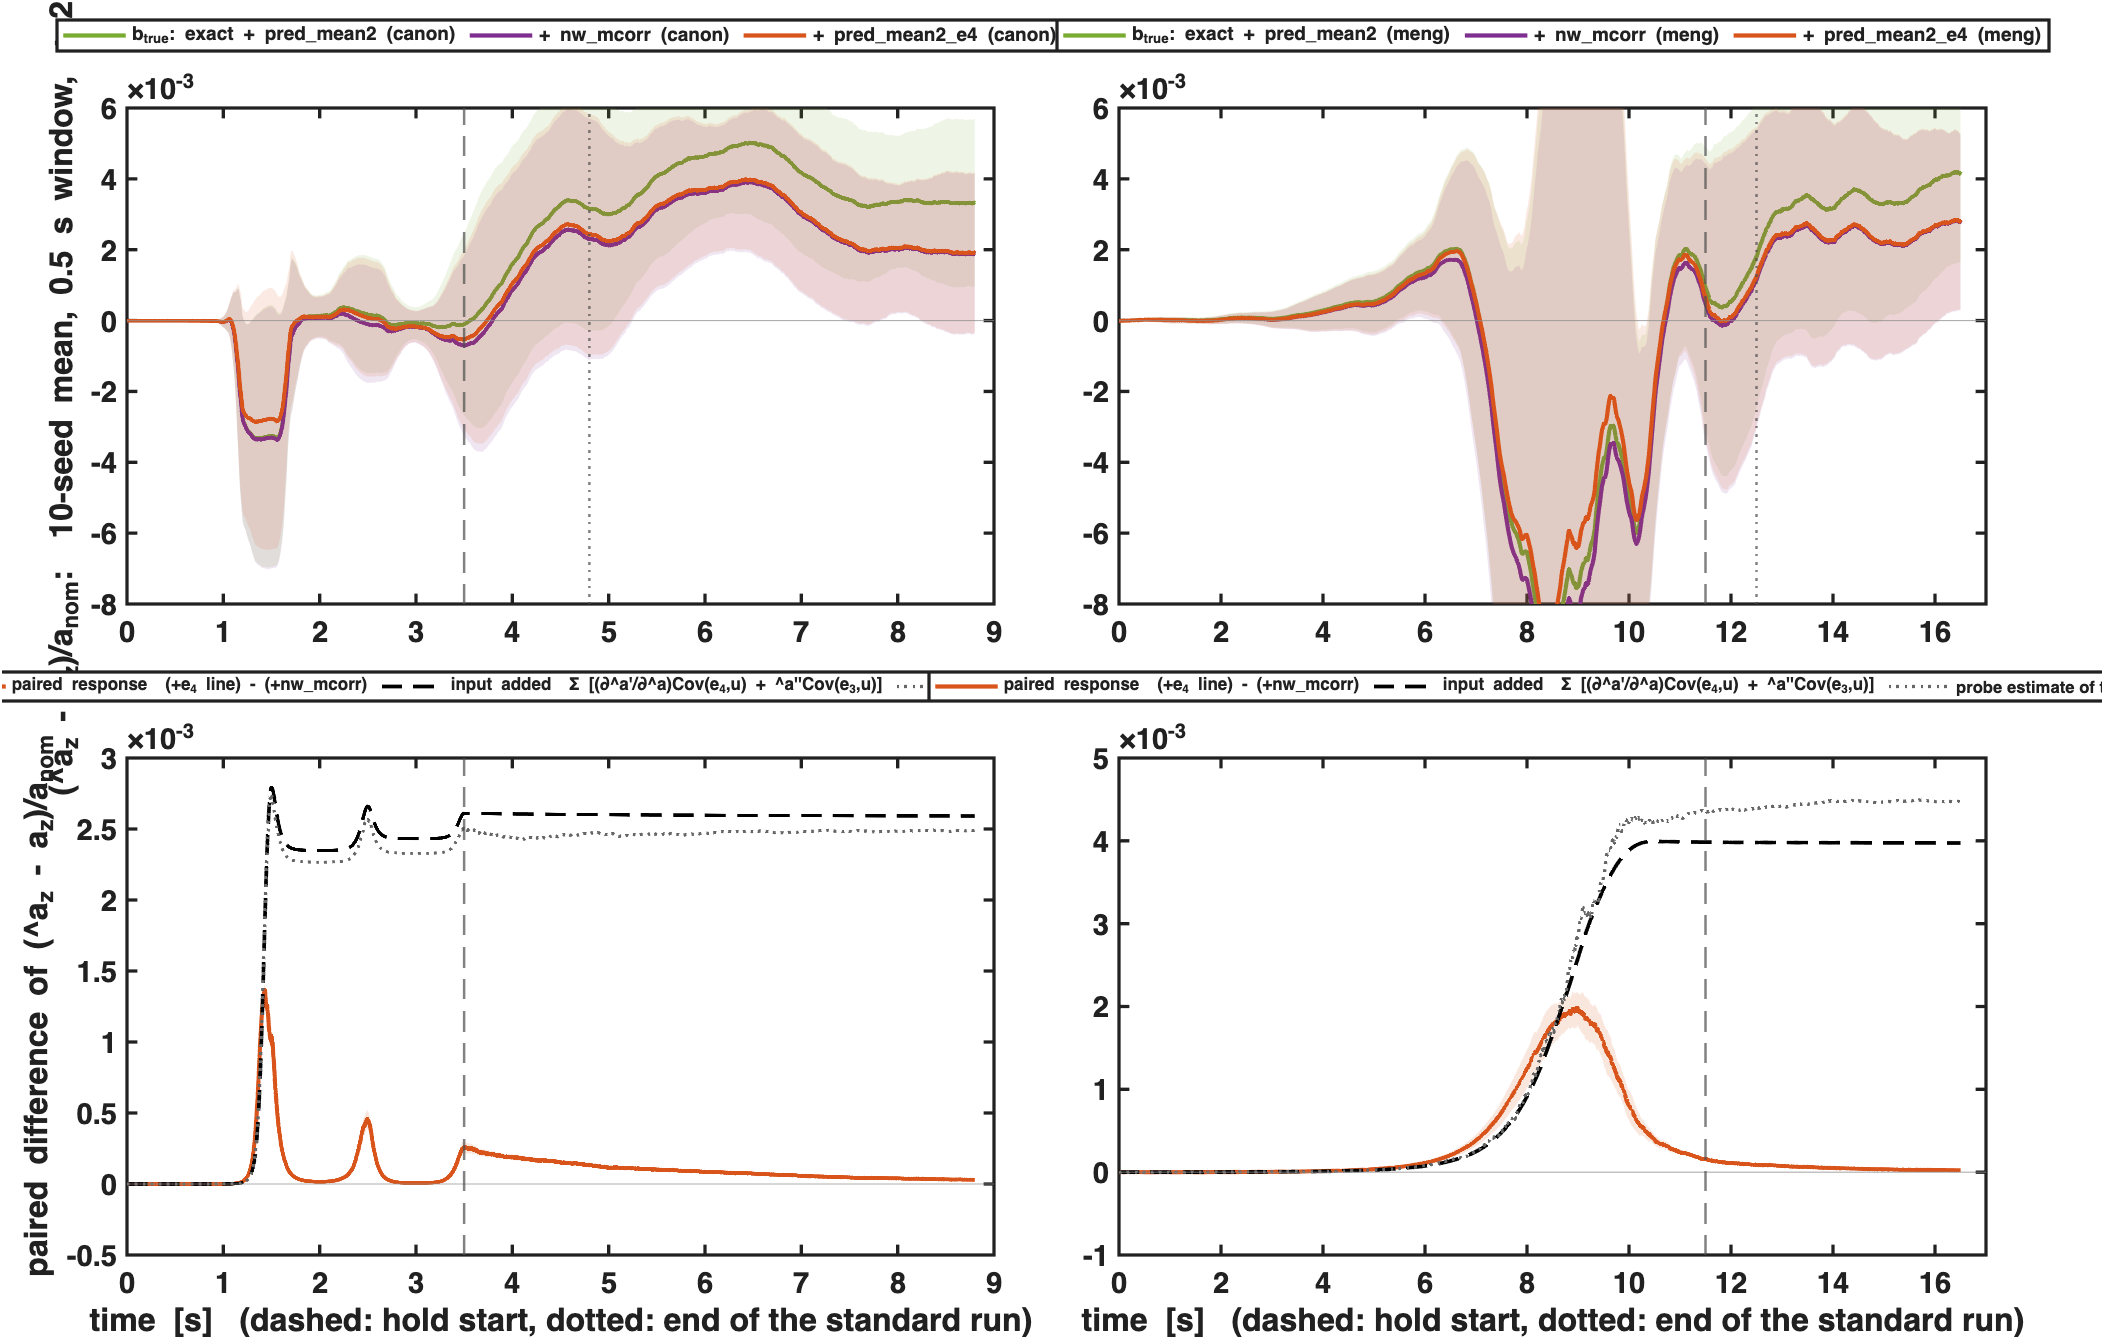
\includegraphics[width=\textwidth]{figures/btrue_three_arms_band.png}

\end{document}
